\begin{figure*}[t]
  \centering
  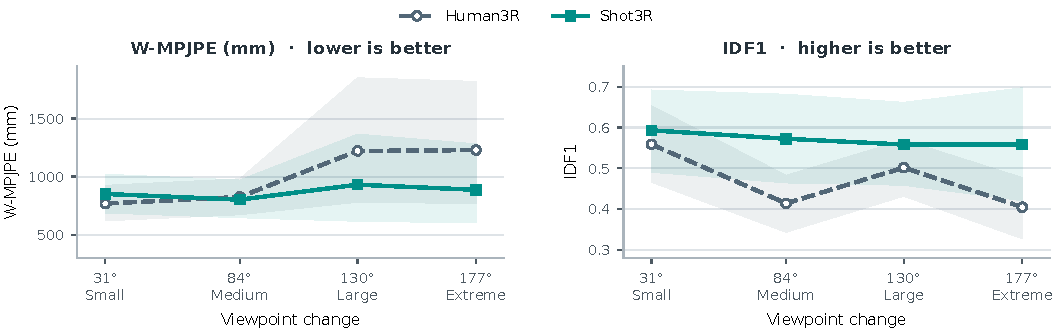
\includegraphics[width=0.82\textwidth]{figures/egohumans_angle_strata.pdf}
  % 中文图注：EgoHumans 中随镜头视角变化的重建和身份表现。曲线给出四个固定视角区间内的
  % W-MPJPE 和 IDF1 绝对值，阴影为以 capture 为单位 bootstrap 得到的 95% 置信区间。
  % Shot3R 在全部区间均获得更高 IDF1，并在 130° 与 177° 的大视角区间明显降低 W-MPJPE。
  \caption{\textbf{Viewpoint response on EgoHumans.} Curves report absolute
  W-MPJPE and IDF1 in four fixed angle strata; bands are capture-bootstrap 95\%
  confidence intervals. \method{} improves IDF1 throughout, with the clearest
  W-MPJPE reductions at $130^\circ$ and $177^\circ$.}
  \label{fig:angle-strata}
\end{figure*}
